\documentclass[10pt,twocolumn,letterpaper]{article}

% Mis propias cosas
\usepackage{booktabs}
% \usepackage{caption}
% \captionsetup[table]{skip=8pt}   % Solo afecta a las tablas
\usepackage{stfloats}  % Agrega esto al preámbulo
\usepackage{float}

\usepackage{cvpr}
\usepackage{times}
\usepackage{epsfig}
\usepackage{graphicx}
\usepackage{amsmath}
\usepackage{amssymb}

% Incluye otros paquetes aquí, antes de hyperref.

% Si comentas hyperref y luego lo descomentas, deberías borrar
% egpaper.aux antes de volver a ejecutar latex.  (O simplemente pulsa 'q' en el primer latex
% run, let it finish, and you should be clear).
\usepackage[breaklinks=true,bookmarks=false]{hyperref}

\cvprfinalcopy % *** Uncomment this line for the final submission

\def\cvprPaperID{****} % *** Enter the CVPR Paper ID here
\def\httilde{\mbox{\tt\raisebox{-.5ex}{\symbol{126}}}}

% Las páginas están numeradas en modo de envío y sin numerar en la versión final
%\ifcvprfinal\pagestyle{empty}\fi
\setcounter{page}{1}
\begin{document}

%%%%%%%%% TITLE
\title{Cartilla Basada en Datos sobre ECDO Parte 1/2: Comprensión Actual de la Teoría de Oscilación de Desacoplamiento Núcleo-Manto Exotérmica Dzhanibekov (ECDO) “Vuelco de la Tierra”}

\author{Junho\\
Publicado en febrero de 2025\\
Sitio web (Descargue los artículos aquí): \href{https://sovrynn.github.io}{sovrynn.github.io}\\
Repositorio de Investigación ECDO: \href{https://github.com/sovrynn/ecdo}{github.com/sovrynn/ecdo}\\
{\tt\small junhobtc@proton.me}
% Para un artículo cuyos autores pertenecen todos a la misma institución,
% omita las siguientes líneas hasta el cierre de ``}''.
% Se pueden añadir autores y direcciones adicionales con ``\and'',
% igual que para el segundo autor.
% Para ahorrar espacio, use la dirección de correo electrónico o la página web, pero no ambas
% \and
% xxx
% Institución2\\
% Primera línea de la dirección de la institución 2\\
% {\tt\small secondauthor@i2.org}
}

\maketitle
%\thispagestyle{empty}

%%%%%%%%% ABSTRACT
\begin{abstract}
En mayo de 2024, un autor en línea con el seudónimo “The Ethical Skeptic” \cite{0} compartió una teoría innovadora llamada Desacoplamiento Exotérmico Núcleo-Manto y Oscilación de Dzhanibekov (ECDO) \cite{1}. Esta teoría sugiere que la Tierra ha experimentado previamente cambios repentinos y catastróficos en su eje de rotación, provocando inundaciones masivas en todo el mundo al derramarse los océanos sobre los continentes debido a la inercia rotacional. Además, presenta un proceso geofísico explicativo y datos que indican que otro cambio de este tipo podría ser inminente. Si bien las predicciones cataclísmicas de inundaciones y del fin del mundo no son nuevas, la teoría sobre ECDO es especialmente convincente debido a su planteamiento científico, moderno, multidisciplinario y basado en datos.

Este artículo es la primera parte de un resumen de dos partes de seis meses de investigación independiente \cite{2,20} sobre la teoría de ECDO theory. Esta resalta tres puntos clave:

\begin{flushleft}
\begin{enumerate}
    \item Un 'giro de la Tierra' similar al propuesto por la ECDO ha ocurrido múltiples veces en la historia reciente de la humanidad, como lo evidencian los mitos del diluvio y señales geológicas de inundaciones continentales extensas.
    \item Se puede determinar la dirección y magnitud aproximadas de los giros de la Tierra pasados.
    \item Datos recientes geomagnéticos y geofísicos sugieren que otro giro de la Tierra podría ser inminente, y que el cambio climático podría ser causado por cambios profundos dentro de la Tierra en lugar de por los humanos.
\end{enumerate}
\end{flushleft}

Además, cubro la física causal detrás de un “giro de la Tierra” propuesto por la teoría ECDO.

En este artículo, me mantengo objetivo enfocándome en datos sólidos, evito las partes convincentes pero especulativas de la teoría, y enfatizo que este es un tema que la humanidad debe investigar con urgencia.
\end{abstract}

%%%%%%%%% BODY TEXT
\section{Introducción}

Las historias de un gran diluvio no son nuevas; de hecho, se encuentran en todas las principales culturas del mundo, abarcando todas las cunas de la civilización. Al graficar (Figura \ref{fig:1}) una compilación de 267 relatos de inundaciones \cite{3}, se muestra que prácticamente todas las áreas habitadas de la Tierra contienen historias de diluvios.

% \begin{figure}[h]
% \begin{figure}[b]
\begin{figure}[h]
\begin{center}
% \fbox{\rule{0pt}{2in} \rule{0.9\linewidth}{0pt}}
   \includegraphics[width=1\linewidth]{b.png}
\end{center}
   \caption{Ubicaciones de historias de inundaciones alrededor del mundo \cite{3}.}
\label{fig:1}
\label{fig:onecol}
\end{figure}

Una mirada más cercana a estas historias de inundaciones nos muestra que no se trató de inundaciones ordinarias, sino de cataclismos destructivos acompañados de inundaciones que limpiaron los continentes.

\subsection{Historias de cataclismos de los nativos americanos}

Las historias de los nativos americanos contienen algunos de los relatos más vívidos de los grandes cataclismos de la Tierra. Los hopi, una tribu nativa americana que vive en el noreste de Arizona, dicen que, \textit{"...Sótuknang llamó a las Personas Hormiga para que abrieran su mundo subterráneo para el pueblo elegido. Cuando estuvieron a salvo bajo tierra, Sótuknang ordenó a los gemelos, Pöqánghoya y Palöngawhoya, que abandonaran sus puestos en los extremos norte y sur del eje del mundo, donde estaban estacionados para mantener la tierra girando correctamente. \textbf{Los gemelos apenas habían abandonado sus estaciones cuando el mundo, sin nadie que lo controlara, perdió el equilibrio, giró locamente, y luego rodó dos veces.} Las montañas se sumergieron en los mares con un gran chapoteo, los mares y lagos se derramaron sobre la tierra; y mientras el mundo giraba a través del espacio frío y sin vida, se congeló hasta convertirse en hielo sólido"} \cite{4}.

Muchas de estas historias describen con precisión la escala masiva de las inundaciones, relatando cómo los océanos subieron hasta cubrir todas las cumbres montañosas, excepto las más altas. Los indios skokomish, que viven en el estado de Washington, cuentan cómo, \textit{"El Gran Espíritu, enojado por la maldad de la gente y los animales, decidió deshacerse de la tierra de todos menos los animales buenos, un hombre bueno y su familia. Por orden del Gran Espíritu, el hombre disparó una flecha hacia una nube, luego otra flecha hacia esa flecha, y así sucesivamente, haciendo una cuerda de flechas desde la nube hasta el suelo. Los animales buenos y la gente subieron. Los animales malos y las serpientes empezaron a subir, pero el hombre rompió la cuerda. \textbf{Entonces el Gran Espíritu causó muchos días de lluvia, inundando hasta la línea de nieve de Takhoma (Monte Rainier).} Después de que toda la gente mala y los animales se ahogaron, el Gran Espíritu detuvo la lluvia, las aguas bajaron lentamente, y la gente y animales buenos bajaron"} \cite{3}. Como referencia, el Monte Rainier es un volcán activo en Washington con una altitud máxima de 4392,5 m sobre el nivel del mar.

La historia de la inundación de los indios Makah del estado de Washingston menciona específicamente una inundación multifase de aguas "muy cálidas", indicando que esta no era una inundación normal: \textit{"El océano subió lo suficiente como para aislar el cabo. Luego se retiró, llegando a su marea más baja cuatro días después, dejando la Bahía Neah completamente seca. Luego volvió a subir para cubrir todo excepto las cimas de las montañas. \textbf{Las aguas que subían estaban muy cálidas.} Las personas con canoas cargaron sus pertenencias y fueron llevadas muy lejos hacia el norte. Muchos murieron cuando sus canoas quedaron atrapadas en los árboles. El mar regresó a la normalidad después de cuatro días más, y las personas se encontraron muy al norte, donde sus descendientes aún viven"} \cite{3}.

\subsection{Historias de cataclismos chinos}

Al otro lado del Océano Pacífico, se dice que la civilización china moderna comenzó con una gran inundación. La dinastía Xia, que se estima existió alrededor del año 2000 a.C., fue fundada por Yu el Grande, quien detuvo la Gran Inundación de Gun-Yu \cite{6}. Durante su tiempo, \textit{"... se dice que ocurrió el milagro de que el sol durante un lapso de diez días no se puso, los bosques se incendiaron y apareció una multitud de abominables alimañas... Una ola inmensa "que alcanzaba el cielo" cayó sobre la tierra de China. \textbf{"El agua llegaba hasta las altas montañas y las estribaciones no podían verse en absoluto"}... "Destructivas en su desbordamiento son las aguas de la inundación", dijo el emperador. "En su vasta extensión abrazan las colinas y sobrepasan las grandes alturas, amenazando los cielos con sus aguas." El emperador ordenó que se hicieran todos los esfuerzos para abrir salidas para las aguas que estaban atrapadas en los valles entre las montañas. Durante muchos años la población trabajó tratando de liberar las llanuras y los valles de las aguas de la inundación cavando canales y drenando los campos. Durante un considerable número de años todos los esfuerzos fueron en vano. El ministro encargado de esta urgente e inmensa labor, Khwan, fue condenado a muerte por su fracaso... y solo su hijo Yu logró drenar la tierra. Este logro fue tan valorado que Yu se convirtió en emperador de China después de Shun, primer sucesor de Yahou"} \cite{5}.

Parecería que no solo China fue inundada, sino que hubo necesidad de recalibrar los puntos cardinales y los movimientos del sol y la luna, lo que implica que la rotación de la Tierra pudo haber cambiado durante la inundación: \textit{\textbf{"Este emperador envió eruditos a diferentes partes de China, e incluso a Indochina, para averiguar la ubicación del norte, oeste, este y sur observando la dirección del amanecer y el atardecer y el movimiento de las estrellas.} También encargó a sus astrónomos que averiguaran la duración de las estaciones y elaboraran un nuevo calendario... "Entonces Yaou [Yahou] ordenó a He y Ho, en reverente acuerdo con los vastos cielos, calcular y delinear los movimientos y apariciones del sol, la luna, las estrellas y los espacios zodiacales; y transmitir respetuosamente las estaciones al pueblo""} \cite{5}.

Los registros de cataclismos en la historia china en realidad se remontan mucho antes de la dinastía Xia, llegando tanto tiempo atrás como en el período de los Tres Soberanos y Cinco Emperadores \cite{7}. Nüwa, una de los Tres Soberanos y figura central en la Creación de la historia china, detuvo la inundación durante un cataclismo en el que la Tierra cambió su rotación: \textit{"Hubo una disputa entre dos de los dioses más poderosos, y decidieron resolverla con una pelea. Cuando el dios del agua Gong Gong vio que estaba perdiendo, golpeó su cabeza contra el Monte Buzhou, un pilar que sostenía el cielo. \textbf{El pilar colapsó y provocó que el cielo se inclinara hacia el noroeste y la tierra se desplazara al sureste.} Esto causó grandes calamidades, como incendios interminables, enormes inundaciones y la aparición de fieras devoradoras de hombres. Nüwa cortó las patas de una tortuga gigante y las usó para reemplazar el pilar caído, aliviando la situación y sellando el cielo roto con piedras de siete colores diferentes, pero no pudo corregir completamente la inclinación del cielo"} \cite{8}.

\subsection{Historias de cataclismos europeos, mayas, medio orientales y del sudeste asiático}

Como hay demasiadas historias de cataclismos para detallar en este trabajo, incluiré una breve mención de algunas de las otras culturas notables con tales relatos. La literatura griega contiene tres historias de inundaciones, la de Deucalión, Ogyges y Dárdano \cite{9,10}. Durante la primera, \textit{"después de nueve días de inundación, el mundo fue destruido, y el arca descansó en la cima del Monte Parnaso"}, cuya cumbre tiene una elevación máxima de 2.457 metros \cite{11}. La literatura maya cree que hubo cuatro Soles distintos antes del Sol actual, y que la era del cuarto Sol, Calchiuhtlicue, terminó con una inundación que destruyó el mundo alrededor del año 3100 a.C. y el nacimiento del actual quinto sol \cite{12}. En el Medio Oriente, la cronología bíblica contiene el famoso diluvio de Noé, y la Epopeya de Gilgamesh, un poema babilónico, cuenta una historia similar \cite{13}. Las culturas del sudeste asiático también son ricas en relatos de inundaciones; por ejemplo, el pueblo Ot Danum de Indonesia dice que, \textit{"un gran diluvio una vez ahogó a muchas personas. Unos pocos sobrevivieron escapando en barcos a la única cima de montaña que quedaba sobre el agua. Vivieron allí durante tres meses hasta que la inundación retrocedió"} \cite{3}. La isla de Borneo, en la que habitan, tiene una elevación máxima de 4.095 metros.

\begin{figure*}[t]
\begin{center}
% \fbox{\rule{0pt}{2in} \rule{.9\linewidth}{0pt}}
\includegraphics[width=1\textwidth]{marine.jpg}
\end{center}
   \caption{Un mapa global de fósiles marinos (oceánicos), sal marina, y salinas/minas de sal \cite{15,16,86,87}.}

   \label{fig:2}
\end{figure*}

\subsection{Análisis Estadístico de Historias de Cataclismos}

Evidentemente, estas historias describen diluvios que a menudo fueron acompañados por otros tipos de fuerzas geofísicas catastróficas. Un análisis de 117 historias de cataclismos (Tabla \ref{tab: 1}) muestra que incendios, cambios topográficos y cambios en la rotación de la Tierra a menudo se registran como ocurridos junto con grandes diluvios \cite{14}:

\begin{table}[ht]
\begin{center}
\renewcommand{\arraystretch}{1.2}  % Opcional, para aumentar el espaciado entre filas
\begin{tabular}{|l|c|c|}
\hline
\textbf{Tipo de Cataclismo} & \textbf{Cantidad} & \textbf{\% de Ocurrencia} \\
\hline\hline
Diluvio/inundación            & 84 & 71.79 \\
Conflagración/incendio        & 39 & 33.33 \\
Cambios topográficos          & 29 & 24.79 \\
Desorden estelar              & 15 & 12.82 \\
Colapso del cielo             & 15 & 12.82 \\
Oscuridad prolongada          & 14 & 11.97 \\

Tierras y lagos perdidos    & 12 & 10.26 \\
Vientos ciclónicos          & 10 & 8.55  \\
Cambios axiales/rotacionales & 9 & 7.69  \\
Ríos/lagos/océanos hirvientes & 8 & 6.84 \\
\hline
\end{tabular}
\end{center}
\caption{Ocurrencias de efectos catastróficos en relatos}
\label{tab: 1}
\end{table}

La especificidad de los relatos de inundaciones provenientes de una multitud de culturas independientes en todo el mundo, junto con relatos coincidentes de otras ocurrencias cataclísmicas, sugiere que estos relatos sobre inundaciones pueden ser relatos directos de desastres que realmente ocurrieron.

\section{Evidencia física de una inundación oceánica}

Corroborando los relatos de inundaciones se encuentran varias formas de evidencia física de una amplia inundación oceánica presentes en la superficie de los continentes terrestres. Las formas más directas de dicha evidencia incluyen sal (agua salada, salinas y minas de sal) y fósiles marinos (oceánicos), que cubren grandes áreas de la masa continental terrestre. La Figura \ref{fig:2} muestra un gráfico de agua salada (azul), salinas y minas (marrón), y fósiles marinos \cite{15,16,86,87}, ilustrando la extensión de estos indicadores de inundación oceánica.

Algunas de las áreas más interesantes que contienen agua salada son las tierras altas del Himalaya en el Tíbet y la cordillera de los Andes en Sudamérica, ambas con una altitud promedio de 4000 metros, la primera representada en la Figura \ref{fig:3}. Los relatos de inundaciones del Tíbet dicen que, \textit{"\textbf{El Tíbet fue casi totalmente inundado}, hasta que el dios Gya tuvo compasión de los sobrevivientes, desvió las aguas hacia Bengala, y envió maestros para civilizar al pueblo, que hasta entonces no era mucho mejor que los monos"} \cite{3}. Los mitos peruanos describen la formación de montañas en conjunto con inundaciones que cubrían las cimas: \textit{"El pastor y sus seis hijos reunieron toda la comida y ovejas que pudieron y las llevaron a la cima de la altísima montaña Ancasmarca. \textbf{A medida que subía el agua de la inundación, la montaña se elevaba, por lo que su cima nunca quedó sumergida, y más tarde la montaña descendió junto con el agua.} Los seis hijos repoblaron la provincia después de la inundación"} \cite{3}.

\begin{figure}[t]
\begin{center}
% \fbox{\rule{0pt}{2in} \rule{0.9\linewidth}{0pt}}
   \includegraphics[width=1\linewidth]{tibet.jpg}
\end{center}
   \caption{Un mapa topográfico del Himalaya que muestra agua salada (verde azulado), sal seca (blanco) y fósiles marinos (rojo) \cite{15,16,86,87}.}
\label{fig:3}
\label{fig:onecol}
\end{figure}

Mientras la escuela uniformista del pensamiento geológico atribuye anomalías como la sal y los fósiles marinos a procesos prolongados que ocurren durante millones de años, los relatos sobre inundaciones de la humanidad deberían llevarnos a cuestionar esa línea de pensamiento. Si el océano realmente cubrió los continentes, entonces el agua salada y los fósiles marinos, fácilmente descubiertos en vastas extensiones de tierras de gran altitud, son exactamente lo que se esperaría encontrar.

\begin{figure*}[t]
\begin{center}
\includegraphics[width=0.85\textwidth]{khafre.jpg}
\end{center}
   \caption{Un diagrama que muestra la erosión kárstica diferencial y con patrones causada por un aumento sostenido y temporal del nivel del mar \cite{27}.}
\label{fig:4}
\end{figure*}

\subsection{Anomalías físicas adicionales}

Existen otras numerosas formas de anomalías que la ciencia uniformista no puede explicar. Perfectamente conservados mamuts congelados de forma instantánea enterrados en barro, con carne aún comestible después de miles de años \cite{17,18,19}, enormes capas de sedimentos apilados y depositados horizontalmente en Norteamérica que abarcan 2.4 millones de km$^2$ \cite{21}, paisajes de megaondas de corriente \cite{22}, y piedras erráticas originadas a cientos de kilómetros de distancia posadas en la cima de montañas \cite{23,26} son solo algunos de los fenómenos que la geología uniformista moderna simplemente descarta con explicaciones generalizadas de "procesos largos y prolongados". Tales anomalías se explican mejor a través de fuerzas geofísicas catastróficas, y se exploran en la segunda parte de este documento.

Adicionalmente, las excursiones geomagnéticas y reversiones del polo son ampliamente aceptadas como un fenómeno recurrente de la Tierra, basado en datos paleomagnéticos \cite{35,40,41}. Sin embargo, la ciencia moderna no logra explicar exactamente por qué y cómo ocurren estos cambios de polaridad.

\section{ECDO y las Pirámides de Guiza}

Las pirámides de Kefrén y Keops en Guiza son uno de los puntos clave en la tesis ECDO de Ethical Skeptic \cite{27}, ya que no solo proporcionan evidencia de una inundación oceánica temporal sostenida, sino que también señalan la posible dirección de los giros ECDO de la Tierra, sugiriendo que nuestros antepasados podían medir los cataclismos terrestres y tenían las habilidades de ingeniería para incrustar este conocimiento en estructuras de piedra masivas y altamente sofisticadas. Estas dos pirámides, supuestamente construidas alrededor del 2500 a.C. como tumbas para los faraones Keops y Kefrén, se encuentran en el norte de Egipto aproximadamente en (30 N, 31 E). Sus bases superan los 200 metros de largo y tienen alrededor de 140 metros de altura. La pirámide de Keops fue construida utilizando aproximadamente 2.3 millones de bloques de piedra caliza, cada uno con un peso promedio de más de dos toneladas \cite{24, 25}.

Existe una gran incertidumbre acerca de los orígenes de estas pirámides, tema que Ethical Skeptic aborda en su tesis. Él señala numerosas inconsistencias en la narrativa convencional que rodea a las pirámides, sugiriendo, en el mejor de los casos, una confusión significativa sobre la edad e historia de las pirámides:

\begin{flushleft}
\begin{itemize}
    \item La datación por carbono de morteros antiguos y herramientas de saqueadores de tumbas cercanos indica que las pirámides probablemente fueron construidas mucho antes de lo convencionalmente creído.
    \item Las llamadas marcas de cantera encontradas en las cámaras internas de la pirámide de Keops son sospechosas en cuanto a su ubicación, material, estado de conservación, uso de jeroglíficos egipcios y momento/naturaleza del descubrimiento, lo que indica que pueden ser falsificaciones. También difieren de otras marcas auténticas de ocre antiguo encontradas en otra parte de la pirámide.
    \item La erosión kárstica diferencial en la cercana Esfinge no concuerda con la narrativa convencional sobre su construcción.
\end{itemize}
\end{flushleft}

\begin{figure*}[t]
\begin{center}
\includegraphics[width=0.85\textwidth]{shafts.jpg}
\end{center}
   \caption{Los conductos y cámaras interiores de la Pirámide de Keops, que Ethical Skeptic propone fue un observatorio geofísico tripartito para la monitorización de eventos ECDO \cite{28}.}
\label{fig:5}
\end{figure*}

Una de las áreas clave de investigación en la tesis de Ethical Skeptic es la erosión diferencial y en patrones en el exterior de la Pirámide de Kefrén, mostrada en la Figura \ref{fig:4}. La punta de la pirámide mantiene su revestimiento original de piedra caliza blanda de Tura, que en su momento cubría toda la pirámide. Esta punta de revestimiento de piedra caliza está ligeramente erosionada, pero se encuentra directamente sobre una capa estrecha fuertemente erosionada por carst, que expone la piedra caliza Mokkatam (dureza 7 de Mohs) más dura, utilizada para los bloques estructurales internos de la pirámide. Debajo de esto, el cuerpo de la pirámide conserva una capa de piedra caliza de Tura (dureza 4 de Mohs) fuertemente erosionada por carst. El punto clave aquí es que la piedra caliza más blanda de Tura usada en el revestimiento externo de la pirámide, que consiste en CaCO$_3$, puede disolverse en agua bajo las condiciones adecuadas. Ethical Skeptic cita la capa de erosión carstica selectiva y severa terminando en la piedra caliza dura de Mokkatam, la erosión en patrón de ondas en las esquinas de la punta, y la diferencia entre la leve erosión de la punta elevada y la intensa erosión carstica del cuerpo inferior de la pirámide, como una evidencia clara de un aumento sostenido del nivel oceánico que también retrocedió rápidamente \cite{27}.

Ethical Skeptic también se centra intensamente en el diseño interno y el estado de la pirámide de Keops (Figura \ref{fig:5}) en su investigación \cite{28}. La pirámide de Keops contiene varias cámaras (la del Rey, la de la Reina y la Subterránea), varios corredores y conductos, así como dos pares de los llamados "conductos de aire", con un par que irradia desde la Cámara del Rey y otro par desde la Cámara de la Reina \cite{29,30}. En este artículo, solo cubriremos las partes más críticas de la investigación de Ethical Skeptic: la orientación y el diseño de los dos pares de "conductos de aire", ya que estos codifican información importante sobre la dirección de los cambios ECDO de la Tierra.

La clave aquí es entender que los conductos fueron construidos para apuntar de manera muy precisa hacia ciertas direcciones. Primero, ambos pares de conductos actualmente apuntan directamente al norte y al sur. Además, cada uno fue construido con un ángulo interno de 104 grados.

Sin embargo, la pista más reveladora es un mapa estelar celeste tallado en el interior de uno de los conductos de la Reina. Este mapa estelar está centrado en una orientación del polo norte celeste de aproximadamente 9600 a 9200 a.C., según la precesión de los equinoccios \cite{28}. Esto sugiere una orientación deliberada de los conductos, y que en la época de la construcción, un par de conductos de las cámaras del Rey y la Reina apuntaban hacia el polo norte celeste. Esto nos lleva a la pregunta: ¿hacia dónde apuntan los otros extremos de los conductos y por qué ambos fueron construidos con un ángulo de 104 grados? Ethical Skeptic propone que éstos fueron hechos para alinearse con el polo norte celeste tras un giro ECDO de 104 grados.

\begin{figure*}[t]
\begin{center}
% \fbox{\rule{0pt}{2in} \rule{.9\linewidth}{0pt}}
\includegraphics[width=1\textwidth]{drawing.jpg}
\end{center}
   \caption{Una representación de la rotación ECDO propuesta yendo 104 grados al norte a lo largo del meridiano 31° E, con cruces que representan los pivotes oriental y occidental y un marcador rojo representando la Pirámide de Keops.}
\label{fig:6}
\end{figure*}

\section{Evidencia de una Rotación de 104 Grados a lo Largo del Meridiano 31}

Ethical Skeptic propone así que la Tierra experimenta vuelcos recurrentes de 104 grados a lo largo del meridiano 31, sobre el cual se encuentran la Pirámide de Keops y sus conductos duales. La Figura \ref{fig:6} muestra la rotación predicha, junto con los "pivotes" este (Indonesia, 121 grados E) y oeste (Sudamérica, 59 grados O), las dos ubicaciones que no cambiarían de posición tras un vuelco a lo largo del meridiano 31. Después de que la Tierra rota a este nuevo estado, se espera que permanezca allí brevemente (unas décadas o siglos) antes de volver a su estado "normal" actual \cite{150}.

Una historia de cataclismo especialmente relevante es contada por Heródoto, el historiador más famoso de la antigua Grecia, quien vivió en el siglo V a.C. \cite{31}. En su libro "Historia de Egipto", Heródoto relata cómo los sacerdotes egipcios le dijeron, \textit{"...desde el primer rey hasta este sacerdote de Hefesto que reinó el último, hubo trescientas cuarenta y una generaciones de hombres... pero trescientas generaciones de hombres equivalen a diez mil años, pues cien años equivalen a tres generaciones... Así, en el periodo de once mil trescientos cuarenta años dijeron que no se había presentado ningún dios en forma humana; ni antes de ese tiempo ni después, entre los restantes reyes que surgieron en Egipto, informaron que algo semejante hubiese ocurrido. \textbf{En este tiempo dijeron que el sol se movió cuatro veces de su lugar habitual de salida, y donde ahora se pone, desde allí dos veces tuvo su salida, y en el lugar de donde ahora sale, allí tuvo dos veces su puesta;} y mientras tanto, nada en Egipto había cambiado de su estado habitual, ni lo que viene de la tierra ni lo que viene del río, ni lo que concierne a enfermedades o muertes"} \cite{32}. El sacerdote de Hefesto puede fecharse a principios del siglo VII a.C., ya que fue contemporáneo a Senaquerib, el rey del Imperio Neoasirio, tal como menciona el propio Heródoto \cite{32,33,34}.

Esta historia es importante porque nos dice que cuando el Sol se movió en Egipto, \textit{específicamente intercambió su lugar de salida y puesta}. Esto solo podría ocurrir si Egipto se volcara 180 grados y permaneciera en una latitud similar. Al considerar el diseño de las pirámides y los datos tratados en la siguiente subsección, podemos inferir que Egipto puede encontrarse en el meridiano a lo largo del cual la Tierra rota a su nueva posición (el meridiano 31 este).

Egipto es el \textit{único} lugar en la Tierra con una historia que menciona que el Sol intercambió específicamente su lugar de salida y puesta. De hecho, la única otra historia en la Tierra que detalla una dirección específica de rotación de la Tierra es la historia de Nüwa de China, que dice que, \textit{"El pilar colapsó y causó que el cielo se inclinara hacia el noroeste y la tierra se moviera al sureste"} \cite{8}. Esta dirección de rotación también concuerda con la dirección de rotación propuesta.

\begin{figure}[t]
\begin{center}
% \fbox{\rule{0pt}{2in} \rule{0.9\linewidth}{0pt}}
   \includegraphics[width=0.95\linewidth]{laj.jpg}
\end{center}
   \caption{Trayectorias de polos geomagnéticos virtuales para (a) la excursión de la Cuenca de Islandia y (b) la excursión de Laschamp \cite{35}.}
\label{fig:7}
\label{fig:onecol}
\end{figure}

\begin{figure*}[t]
\begin{center}
% \fbox{\rule{0pt}{2in} \rule{.9\linewidth}{0pt}}
\includegraphics[width=0.95\textwidth]{biodiversity.jpg}
\end{center}
   \caption{Una representación de los principales desiertos del mundo y los alternantes focos de biodiversidad \cite{28}.}
\label{fig:9}
\end{figure*}

\begin{figure}[t]
\begin{center}
% \fbox{\rule{0pt}{2in} \rule{0.9\linewidth}{0pt}}
   \includegraphics[width=1\linewidth]{meinesz3.jpg}
\end{center}
   \caption{Una representación de los patrones de cizalla en la corteza terrestre \cite{36}.}
\label{fig:8}
\label{fig:onecol}
\end{figure}

\subsection{Evidencia Física de una Rotación de 104 Grados a lo Largo del Meridiano 31}

La evidencia física que respalda esta dirección de rotación incluye datos paleomagnéticos, tectónicos, del desierto, de biodiversidad, paleocorrientes y de erráticos glaciares.

Un estudio de los datos paleomagnéticos que preservan las rutas del polo geomagnético durante las excursiones de la Cuenca de Islandia y Laschamp \cite{35}, representado en la Figura \ref{fig:7}, muestra los polos rotando aproximadamente alrededor del pivote oriental ECDO de (0 N, 121 E). Estos datos se registran en ciertos tipos de minerales magnéticos en rocas que se formaron durante las excursiones del polo, preservando información sobre la dirección e intensidad del campo magnético terrestre en ese momento.

Un estudio de los planos de cizalladura (fallas) en la corteza terrestre (Figura \ref{fig:8}), donde la corteza de la Tierra se ha fracturado o deformado, también sigue el mismo patrón. Felix Meinesz, un geofísico holandés, explica en su artículo \cite{36} que la razón más probable para este patrón es un cambio en el eje de rotación de la Tierra.

Las ubicaciones de los principales desiertos del mundo y los focos de biodiversidad también se alinean con este patrón. Los desiertos existen en lugares donde se espera que sean inundados fuertemente con sedimentos, mientras que los focos de biodiversidad existen en áreas que no son tan afectadas por el desplazamiento oceánico \cite{28}. Esta alineación se muestra en la Figura \ref{fig:9}.

Estas alineaciones con la trayectoria rotacional ECDO también existen en las paleocorrientes de sedimentos preservadas en las capas de arenisca del oeste de los Estados Unidos \cite{21}, y en los erráticos glaciares, que son rocas que han sido recogidas, supuestamente por glaciares, y depositadas en otro lugar sobre un lecho rocoso de un tipo diferente al de la roca errática. En Gran Bretaña, estos erráticos siguen trayectorias de flujo esperadas consistentes con una rotación ECDO \cite{67,68}.

\section{Física causante detrás de un vuelco ECDO}

\begin{figure*}
\begin{center}
% \fbox{\rule{0pt}{2in} \rule{1\linewidth}{0pt}}
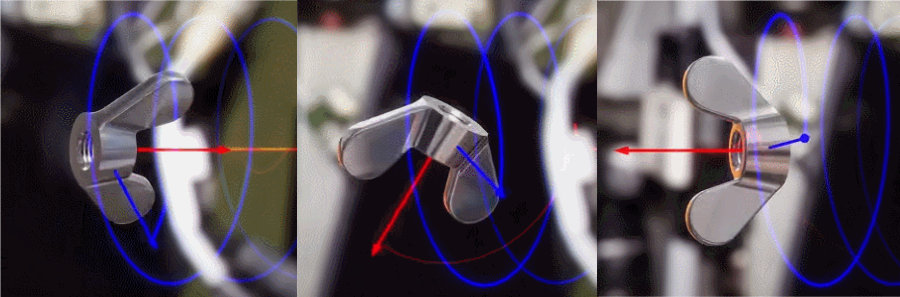
\includegraphics[width=0.9\textwidth]{dzhani.jpg}
\end{center}
   \caption{Una representación del efecto Dzhanibekov \cite{28}.}
\label{fig:10}
\end{figure*}

\begin{figure*}[t]
\begin{center}
% \fbox{\rule{0pt}{2in} \rule{.9\linewidth}{0pt}}
\includegraphics[width=1\textwidth]{layers.jpg}
\end{center}
   \caption{Representación de los procesos internos de la Tierra que llevan al vuelco ECDO \cite{129}.}
\label{fig:11}
\end{figure*}

\begin{figure}[t]
\begin{center}
% \fbox{\rule{0pt}{2in} \rule{0.9\linewidth}{0pt}}
   \includegraphics[width=1\linewidth]{llvp.jpg}
\end{center}
   \caption{Una imagen visual detallada del LLVP bajo Sudáfrica \cite{28}.}
\label{fig:12}
\label{fig:onecol}
\end{figure}

El principio detrás de un cambio rápido en el eje de rotación de la Tierra radica en la física de los objetos en rotación. El ejemplo canónico de esto es el efecto Dzhanibekov, descubierto por el cosmonauta ruso Vladimir Dzhanibekov \cite{37}, y representado en la Figura \ref{fig:10}. Un objeto que no gira perfectamente sobre uno de sus tres ejes principales de inercia no mantendrá un eje de rotación fijo. Si gira cerca de su segundo eje principal, experimentará lo que parecen ser cambios repentinos en la rotación. Si bien esto no es exactamente lo que creemos que sucede durante los cambios rápidos de la Tierra, la cuestión es que en ausencia de fuerzas externas, solo la física de rotación puede explicar un cambio rápido en el eje de rotación de la Tierra.

Para ser precisos, casi con certeza la Tierra no experimenta un efecto Dzhanibekov simple y uniforme. Si este fuera el caso, podríamos detectar un desplazamiento gradual en el eje de rotación de la Tierra a lo largo del tiempo. Más bien, creemos que la Tierra experimenta alteraciones periódicas y repentinas en su estructura física, lo que lleva a un desacoplamiento de su "rotación exterior" (corteza/manto) y sus "cuerpos internos de rotación" (núcleo). Sin una influencia externa, la ley de conservación del momento angular establece que la Tierra no puede cambiar repentinamente su eje de rotación, por lo que un desacoplamiento entre los cuerpos de rotación exteriores e interiores es una de las pocas cosas, salvo un impacto externo en la Tierra, que podría causar un giro repentino y abrupto.

Se cree que el proceso específico que impulsa la alteración interna en la Tierra es un cambio de estado en la estructura del hierro que compone el núcleo terrestre (Figura \ref{fig:11}). El núcleo interno está formado por hierro empaquetado hexagonalmente (Fe) \cite{141}. Cuando este hierro se convierte en un estado líquido metálico, libera energía cinética y es arrojado al núcleo externo. Este cambio de fase reduce la permeabilidad magnética del núcleo, debilitando el campo geomagnético, y libera calor, creando estructuras LLVP (provincias de cizalladura de baja velocidad y gran tamaño) (Figura \ref{fig:12}) \cite{38} en el manto, y calentando la superficie de la Tierra a través de los océanos abisales. Ambas tendencias han sido bien documentadas en los últimos siglos y se discuten más adelante en este trabajo.

Este mismo proceso dentro de la Tierra, ocurriendo de manera inversa, también se cree que impulsa el regreso al estado rotacional actual de la Tierra relativamente poco tiempo después de que ocurre la inversión.

\section{Evidencia de un inminente vuelco de la Tierra}

Hay fuertes razones para creer que estamos al borde de otro vuelco de la Tierra. No ha ocurrido un cataclismo durante varios milenios, lo cual es aproximadamente la frecuencia con la que estos eventos parecen suceder según relatos históricos y datos. Los datos más sólidos que respaldan un vuelco inminente provienen de datos geomagnéticos recientes, que indican que el campo geomagnético de la Tierra se ha estado debilitando durante aproximadamente dos mil años. Este debilitamiento se ha acelerado y ha alcanzado tasas alarmantes en las últimas décadas.

\begin{figure}[t]
\begin{center}
% \fbox{\rule{0pt}{2in} \rule{1\linewidth}{0pt}}
   \includegraphics[width=1\linewidth]{npw.jpg}
\end{center}
   \caption{La posición del polo norte geomagnético desde 1590 hasta 2025, representada en intervalos de 5 años \cite{142}.}
\label{fig:13}
\label{fig:onecol}
\end{figure}

Representado en la Figura \ref{fig:14} está el campo geomagnético de la Tierra en 1590 y 2025 \cite{125,126}. Como se muestra en la figura, el campo se ha debilitado significativamente.

Otro indicador del debilitamiento del campo geomagnético es la posición del polo norte geomagnético (Figura \ref{fig:13}). Históricamente, el polo norte geomagnético se ha ubicado en el Ártico canadiense. Sin embargo, ha estado desplazándose lentamente durante los últimos siglos, y su velocidad se aceleró significativamente hace unas décadas. Actualmente se está moviendo rápidamente hacia Rusia a una velocidad de 55 kilómetros por año \cite{124}.

\begin{figure*}[t]
\begin{center}
% \fbox{\rule{0pt}{2in} \rule{.9\linewidth}{0pt}}
\includegraphics[width=0.9\textwidth]{saa.jpg}
\end{center}
   \caption{Una representación del debilitamiento del campo geomagnético desde 1590 hasta 2025. Calculado utilizando los modelos gufm1 e IGRF-14 \cite{125,126}.}
\label{fig:14}
\end{figure*}

\begin{figure}[t]
\begin{center}
% \fbox{\rule{0pt}{2in} \rule{1\linewidth}{0pt}}
   \includegraphics[width=1\linewidth]{ocean-highlight.jpg}
\end{center}
   \caption{Tasas de calentamiento oceánico profundo ($>$2000 m de profundidad) desde 1991 hasta 2010, señaladas en rojo \cite{132}.}
\label{fig:15}
\label{fig:onecol}
\end{figure}

Se cree que el campo magnético terrestre es generado por un dínamo interno: columnas circulares de corrientes de magma moviéndose en el núcleo externo de la Tierra debido a su rotación \cite{123}. Un debilitamiento del campo geomagnético es un síntoma de perturbaciones en el interior profundo de la Tierra. Según la teoría ECDO, estas perturbaciones expulsan calor y eventualmente conducen al desacoplamiento del manto y el núcleo, causando un vuelco de la Tierra \cite{1}.

Hay datos considerables que corroboran la presencia de procesos endotérmicos en el interior de la Tierra. Una Tierra en calentamiento se documenta en el aumento de las temperaturas superficiales continentales y oceánicas \cite{127,128}, el aumento de los niveles atmosféricos de CO2 moviéndose en sincronía con las plumas de calor terrestre \cite{129,130}, y una disminución en la extensión global del hielo marino \cite{131}. Los datos sugieren que los niveles crecientes de CO2 y las temperaturas no son la causa del cambio climático "provocado por el hombre", sino más bien efectos posteriores de un núcleo exotérmico \cite{129}.

Lo más significativo es que los estudios sobre las tasas de calentamiento en el océano profundo (profundidad $>$2000 metros) muestran que no solo los océanos profundos se están calentando, sino que las tasas de calentamiento más fuertes se encuentran en la capa abisal (4000 - 6000 m). Este calentamiento en las profundidades tiene un centroide por debajo de los 4000 metros \cite{132,129}, lo cual no sería posible si los océanos estuvieran siendo calentados desde arriba por la atmósfera. Dichos datos brindan un fuerte respaldo a la idea de que los cambios recientes en el clima y el campo geomagnético son impulsados por procesos en el interior profundo de la Tierra. La Figura \ref{fig:15} muestra las tasas de calentamiento oceánico profundo global desde 1991 hasta 2010 \cite{132}.

\section{Modelando el inminente vuelco terrestre}

\begin{figure}[t]
\begin{center}
% \fbox{\rule{0pt}{2in} \rule{1\linewidth}{0pt}}
   \includegraphics[width=1\linewidth]{saa-crop.jpeg}
\end{center}
   \caption{Un cálculo de punto de inflexión basado en la Anomalía del Atlántico Sur apunta a una fecha del 13 de marzo de 2059 \cite{125,126}.}
\label{fig:16}
\label{fig:onecol}
\end{figure}

Predecir el momento del próximo vuelco de la Tierra es una tarea compleja. Actualmente, el mejor modelo que tenemos para esto se encuentra en el campo geomagnético de la Tierra: la Anomalía del Atlántico Sur (SAA). Esta región sobre el Atlántico Sur tiene la menor fuerza de campo geomagnético y se define como el área con una fuerza de campo por debajo de 32.000 nanoteslas \cite{135}, que fue el valor más bajo en 1590. El área superficial de la Anomalía del Atlántico Sur aumentó del 1\% de la superficie terrestre en 1590 al 21\% en 2025 \cite{136}.

Para obtener una estimación de cuándo podría ocurrir el vuelco de la Tierra, ajusté los datos de la extensión superficial de la SAA a una ecuación de punto de inflexión de ley de potencias, que modela un sistema complejo acercándose a una transición crítica, en la que el sistema experimenta un cambio brusco y dramático. Mis cálculos arrojaron una fecha de punto de inflexión predicha para el 13 de marzo de 2059 (Figura \ref{fig:16}). Esta predicción se volvería cada vez más precisa a medida que nos acerquemos a la transición \cite{136}.

Otras métricas como la deriva del eje de rotación, anomalías meteorológicas y datos sísmicos y volcánicos también pueden ayudarnos a obtener una mejor predicción de cuándo podría ocurrir el próximo vuelco de la Tierra.

\section{Línea de Tiempo Histórica de los ECDO}

Si bien establecer una línea de tiempo exacta para eventos ECDO pasados es difícil, parece que hubo al menos 2 eventos ECDO durante el Holoceno. Obsérvese el relato contado por Heródoto de parte de los sacerdotes egipcios que, \textit{"desde el primer rey hasta este sacerdote de Hefesto que reinó el último, hubo trescientas cuarenta y una generaciones de hombres... En este tiempo decían que el sol se había movido cuatro veces de su lugar acostumbrado de salida, y donde ahora se pone, desde allí había salido dos veces, y en el lugar de donde ahora sale, dos veces se había puesto"} \cite{32}. Platón, que vivió durante el siglo V a. C. \cite{111}, afirmó que después del diluvio que hundió la Atlántida en un solo día y noche 9.000 años antes, \textit{"desde entonces ha habido muchos diluvios, y los sobrevivientes que quedaron en las montañas ignoraban el arte de la escritura, y durante muchas generaciones se dedicaron por completo a adquirir los medios de subsistencia"} \cite{112}, lo que sugiere que hubo más de dos vuelcos desde el final del Younger Dryas hacia 9700 a. C. La evidencia física presentada a lo largo de este artículo y en mi investigación \cite{2} proporciona abundante evidencia para el relato de Platón.

La fecha candidata más reciente para un vuelco ECDO es durante el período de 2300 a 1600 a.C., al cual se han atribuido muchos relatos de inundaciones cataclísmicas (Gun-Yu \cite{113,114,115}, Ogyges \cite{116,117}, Perú \cite{118,119}, Éxodo \cite{120}), destrucciones y abandonos civilizatorios (Mohenjo-Daro \cite{121}, Creta Minoica\cite{100,101}) y anomalías físicas (eventos Bond \cite{122}, evento de 4.2 milenios \cite{90}). No hay una amplia convergencia de evidencia más reciente que sugiera un evento catastrófico importante.

\section{Conclusión}

La Operación NANOOK fue un esfuerzo de reconocimiento estadounidense durante la Guerra Fría para mapear el Ártico y la costa norte soviética después de la Segunda Guerra Mundial \cite{137}. Durante su investigación, descubrieron que el polo magnético estaba entre 125 y 200 millas al norte de donde se suponía que debía estar según hallazgos de expediciones anteriores. En consecuencia, \textit{"Entre los científicos del gobierno, surgió la pregunta de qué ocurriría cuando los polos magnético y geográfico coincidieran. Para responder esto, bajo el control del proyecto del Dr. Paul A. Siple, la Rand Corporation fue contratada para realizar estudios de laboratorio utilizando modelos de la Tierra construidos por esferas concéntricas – una esfera interna representando el núcleo de hierro fundido electromagnéticamente cargado de la Tierra, cuyo eje definía los polos “magnéticos”; y una esfera externa representando la corteza terrestre que rotaba alrededor de un eje polar “geográfico”. Se determinó, a través de experimentos repetidos, que a medida que el polo “magnético” se aproximaba al polo “geográfico”, el polo “magnético” en cierto punto aceleraría su tasa de convergencia como si fuera atraído hacia el polo “geográfico” por fuerza centrípeta y saltaría para coincidir; pero en vez de coincidir los polos, el polo “magnético” rápidamente se “volcaría” alrededor del polo “geográfico”, luego saldría girando hacia el ecuador como si fuera por fuerza centrífuga, terminando en una posición donde los dos ejes asumen una divergencia de aproximadamente 89 grados. Después de que ocurriera este vuelco polar, los ejes luego comenzarían gradualmente a reconverger durante un largo período de tiempo"} \cite{138,139}.

Posteriormente, \textit{"En una de las reuniones científicas a las que asistió el Mayor White en el Pentágono a principios de 1948, los científicos discutieron la conveniencia de alertar al público sobre el inminente fenómeno de volcamiento polar. Ninguno de los científicos estuvo de acuerdo en ocultar la información al público; pero, por otro lado, tampoco pudieron acordar cómo darla a conocer. El conocimiento de este fenómeno, según algunos, podría por sí solo destruir el tejido moral de la sociedad. Sus temores aparentemente eran infundados cuando, a principios de la década de 1950, la información sobre el fenómeno fue publicada tanto en una columna de periódico como en un artículo de revista, pero sorprendentemente no generó reacción alguna de un público aparentemente atónito, parroquial o incrédulo"} \cite{138,139}.

¿Por qué no prestamos atención a esto? Hay razones suficientes para creer que la Tierra se ha volcado antes. Este artículo, junto con la parte dos, proveen un denso resumen de una gran convergencia de evidencia de muchas áreas que sugiere que este es el caso, tales como relatos de inundaciones por todo el mundo, fósiles de sal y marinos cubriendo los continentes, antiguos refugios subterráneos, restos de animales y paisajes geológicos catastróficos. Se supone que los humanos tienen cientos de miles de años, sin embargo la historia moderna solo se remonta a varios miles de años. ¿No podría ser el caso que de vez en cuando, la Tierra se voltea, los continentes se limpian, y nos vemos forzados a regresar al punto de partida – la Edad de Piedra – reduciendo nuestros registros de la historia antigua a un puñado de relatos cataclísmicos? Si es así, entonces evitar que esto ocurra de nuevo podría ser una de las tareas más importantes de la humanidad.

Para terminar, les dejo este relato recogido en el Timeo, escrito por Platón, de una conversación entre Solón, un estadista ateniense, y sacerdotes egipcios \cite{140}: \textit{"Y en una ocasión, cuando [Solón] quiso llevarlos a hablar sobre historia antigua, intentó contarles la más antigua de nuestras tradiciones, acerca de Foroneo, quien fue considerado el primer hombre, y de Niobe; y continuó relatando la leyenda sobre Deucalión y Pirra después del Diluvio, y cómo sobrevivieron, y dio la genealogía de sus descendientes; y al relatar el número de años ocupados por los eventos mencionados trató de calcular los períodos de tiempo. Entonces uno de los sacerdotes, un hombre prodigiosamente anciano, dijo: “Oh Solón, Solón, ustedes los griegos siempre son niños: no existe tal cosa como un griego viejo.” Y al escuchar esto, él preguntó: “¿Qué quieres decir con esto?” Y el sacerdote respondió: “Son jóvenes en alma, todos ustedes. Porque en eso no poseen ninguna creencia antigua ni derivada de la tradición, ni tampoco una ciencia envejecida con los años. Y esta es la razón: Ha habido y habrá muchas y diversas destrucciones de la humanidad, de las cuales las mayores son por fuego y agua, y las menores por incontables otros medios. En verdad la historia que se cuenta en tu país, así como en el nuestro, de cómo una vez Faetón, hijo de Helios, unció el carro de su padre y, al no poder guiarlo por el curso que tomaba su padre, abrasó todo lo que había sobre la tierra y él mismo pereció por un rayo, esa historia, tal como se cuenta, tiene la apariencia de una leyenda, pero la verdad está en la ocurrencia de un cambio de los cuerpos celestes que giran alrededor de la Tierra, y una destrucción de las cosas sobre la Tierra por un fuego feroz, que se repite a largos intervalos. En esos tiempos todos los que viven en las montañas y lugares altos y secos sufren la destrucción más que aquellos que viven cerca de ríos o el mar; y en nuestro caso el Nilo, nuestro Salvador de otras formas, nos salva también entonces de esta calamidad al elevarse bastante. Y por otro lado, cuando los dioses purifican la Tierra con un diluvio de aguas, todos los pastores y ganaderos que están en las montañas se salvan, pero los que se encuentran en las ciudades de tu tierra son arrastrados al mar por las corrientes; mientras que en nuestro país, ni entonces ni en ningún otro momento el agua desciende sobre nuestros campos desde arriba, al contrario, todo tiende naturalmente a brotar desde abajo. Por eso, por estas razones, lo que aquí se conserva se considera lo más antiguo; la verdad es que en todos los lugares donde no hay calor o frío excesivo para evitarlo, siempre existe alguna población humana, a veces más, a veces menos numerosa. Y si ha ocurrido algún evento que sea noble o grande o de alguna forma notable, sea en tu país o en el nuestro, o en algún otro lugar del que tengamos noticia, todos esos eventos se registran y se preservan aquí en nuestros templos desde tiempos antiguos; mientras que tu pueblo y los demás, cada vez, solo disponen de letras y tales artes como requieren los Estados civilizados, y cuando después del intervalo usual de años, como una plaga, el diluvio del cielo desciende de nuevo sobre los suyos, no deja a ninguno salvo a los incultos y analfabetos, de modo que ustedes vuelven a ser jóvenes, sin conocimiento de todo lo que ocurrió en tiempos antiguos en esta tierra o en la suya. Ciertamente las genealogías que relataste ahora, Solón, respecto al pueblo de tu país, no son mucho mejores que cuentos infantiles; pues, en primer lugar, recuerdas solo un diluvio, aunque muchos han ocurrido previamente; y además, ignoras el hecho de que la raza más noble y perfecta entre los hombres nació en la tierra donde ahora habitas, y de ellos tanto tú mismo como toda tu ciudad existente descienden, de alguna pequeña semilla que quedó viva por casualidad; pero esto ha pasado desapercibido para ti porque durante muchas generaciones los sobrevivientes murieron sin poder expresarse por escrito. Pues en verdad en un tiempo, Solón, antes de la mayor destrucción causada por el agua, lo que ahora es el Estado ateniense fue el más valiente en la guerra y supremamente bien organizado en todos sus aspectos. Se dice que poseía las más espléndidas obras de arte y la más noble organización política de cualquier nación bajo el cielo de la que hayamos escuchado”}.

Estos mismos sacerdotes, por supuesto, también contaron a Solón sobre la antigua civilización de la Atlántida: \textit{"Porque todo lo que tenemos aquí, dentro de la desembocadura de la que hablamos, es evidentemente un puerto con una entrada estrecha; pero aquello es un verdadero océano, y la tierra que lo rodea debe llamarse, en el más pleno y verdadero sentido, un continente. Ahora, en esta isla de la Atlántida existía una confederación de reyes, de gran y maravilloso poder, que dominaba toda la isla, y también muchas otras islas y partes del continente; y, además, de las tierras aquí dentro de los Estrechos gobernaban Libia hasta Egipto, y Europa hasta la Tirrenia. Así que este ejército, al reunirse todo, intentó en una sola acometida esclavizar tanto su país como el nuestro y todo el territorio dentro de los Estrechos. Y fue en ese momento, Solón, cuando el pueblo de tu Estado demostró su valor y poder ante la mirada de todo el mundo. Porque se destacó por encima de todos en gallardía y artes bélicas, y actuando en parte como líder de los griegos, y en parte luchando solo cuando todos los demás lo abandonaron, después de enfrentar los más mortales peligros, derrotó a los invasores y erigió un trofeo; por lo cual salvó de la esclavitud a quienes aún no habían sido esclavizados, y a todos los demás que habitamos dentro de los límites de Hércules nos liberó generosamente. Pero tiempo después ocurrieron terremotos y diluvios portentosos, y les sobrevinieron un terrible día y noche, cuando todo el ejército de sus guerreros fue devorado por la tierra, y la isla de la Atlántida de igual forma fue tragada por el mar y desapareció"}.

\section{Agradecimientos}

Gracias a Ethical Skeptic, el autor original de la tesis ECDO, por completar su perspicaz y revolucionaria tesis y compartirla con el mundo. Su tesis tripartita \cite{1} sigue siendo la obra seminal sobre la teoría de la Desacoplamiento Exotérmico Núcleo-Manto por Oscilación Dzhanibekov (ECDO), y contiene mucha más información sobre el tema de la que he resumido aquí.

Gracias a Ankit, quien procesó los datos de la compilación de cataclismos en la Tabla 1.

Y, por supuesto, gracias a los gigantes cuyos hombros nos sostienen; aquellos que han realizado toda la investigación y el análisis que hicieron posible este trabajo y que trabajaron para traer luz a la humanidad.

\clearpage
\twocolumn

\section{Imágenes Adicionales}

\begin{figure}[H]
\begin{center}
% \fbox{\rule{0pt}{2in} \rule{1\linewidth}{0pt}}
   \includegraphics[width=1\linewidth]{wave.jpg}
\end{center}
   \caption{Una mirada cercana a la erosión ondulada, parabólica y socavada en la pirámide de Kefrén \cite{27}.}
\label{fig:19}
\label{fig:onecol}
\end{figure}

\begin{figure}[H]
\begin{center}

% \fbox{\rule{0pt}{2in} \rule{1\linewidth}{0pt}}
   \includegraphics[width=1\linewidth]{star-stone.jpg}
\end{center}
   \caption{El mapa estelar tallado en piedra en uno de los conductos de la pirámide de Keops \cite{28}.}
\label{fig:20}
\label{fig:onecol}
\end{figure}

\begin{figure*}[t]
\begin{center}
% \fbox{\rule{0pt}{2in} \rule{.9\linewidth}{0pt}}
\includegraphics[width=1\textwidth]{deepsea.jpg}
\end{center}
   \caption{Una visualización de la anomalía de calentamiento oceánico profundo y abisal comparada con una curva de calentamiento oceánico atmosférico normal. La anomalía de calentamiento general ha sido tomada de la NOAA \cite{147}, las distribuciones de calentamiento profundo y abisal de un estudio de Desbruyeres \cite{132}, y el procesamiento y la visualización de los datos por Ethical Skeptic \cite{129}.}
\label{fig:21}
\end{figure*}

\begin{figure*}[t]
\begin{center}
% \fbox{\rule{0pt}{2in} \rule{.9\linewidth}{0pt}}

\includegraphics[width=1\textwidth]{sealevel.jpeg}
\end{center}
   \caption{El nivel del mar muestra un aumento del 20\% en la varianza durante 75 años en 63 estaciones, lo que indica un aumento en la velocidad de la corriente. Las alzas en la varianza del nivel del mar coinciden con pulsos de calor oceánico, lo que indica que ambos pueden ser causados por el calentamiento desde las profundidades bajo los océanos de la Tierra \cite{2,129}.}
\label{fig:22}
\end{figure*}

\begin{figure*}[t]
\begin{center}
% \fbox{\rule{0pt}{2in} \rule{.9\linewidth}{0pt}}
\includegraphics[width=1\textwidth]{co2.jpg}
\end{center}
   \caption{El CO2 atmosférico en ppm ha aumentado de manera constante durante los últimos 45 años, probablemente causado por un aumento en las temperaturas oceánicas. Fuente: NOAA \cite{148,129}.}
\label{fig:23}
\end{figure*}

\begin{figure*}[t]
\begin{center}
% \fbox{\rule{0pt}{2in} \rule{.9\linewidth}{0pt}}
\includegraphics[width=1\textwidth]{ice.jpg}
\end{center}
   \caption{La extensión global del hielo marino se ha estado reduciendo durante los últimos 45 años, debido al calentamiento de la Tierra. Fuente: ADS \cite{149}.}
\label{fig:24}
\end{figure*}

\clearpage
\twocolumn

{\small
\renewcommand{\refname}{Referencias}
\bibliographystyle{ieee}
\bibliography{egbib}
}

\end{document}
